\chapter{Related Work}
The related work will be described here. Need to find out how are large computations handled in other fields and also in the 3D printing field. 
\section{Fields involving large computations}

\section{Introduction to distributed systems and its types}
Distributed system consists of autonomous systems (AS) connected through network which interact (if necessary) through message passing and most importantly give the user an illusion of being single large system \cite{DCE}. The main goal of distributed system is to connect the users and the available infrastructure i.e. IT resources in a transparent, open, cost-effective, reliable as well as scalable way. Transparency in distributed computing environment (DCE) means that the user is unaware of the underlying system complexities in terms of location of the AS, heterogeneity of the system hardware, concurrency and replication of the AS mainly to provide reliability and fault tolerance. Scalability refers to the property by which the number of AS in the DCE can be increased (scaled in) or decreased(scaled out) so as to provide best suited infrastructure to handle the fluctuating load (i.e. the amount of work to be done).The shared resources of the distributed system can be broadly classified as physical resources and virtual resources. The Figure\ref{fig:TypesOfResourceSharing} details the resources included in the two categorizes. 

\begin{figure}[ht!]
\centering
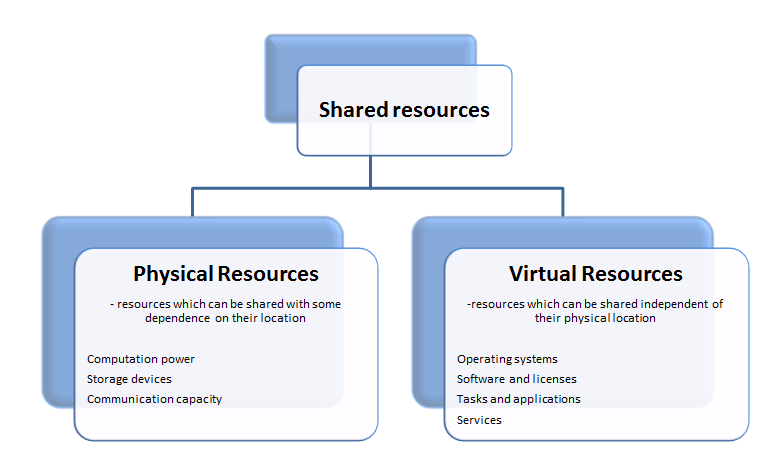
\includegraphics[scale=0.6]{TypesOfResourceSharing.PNG}
\caption{Distributed System Shared Resource Classification}
\label{fig:TypesOfResourceSharing}
\end{figure}
  
Distributed Computing is a vast domain which consists of various different types of computing environments like utility computing (grid computing and cloud computing), cluster computing, peer-to-peer computing and Jungle computing (figure \ref{fig:DistributedComputingEnv}). 

\begin{figure}[ht!]
\centering
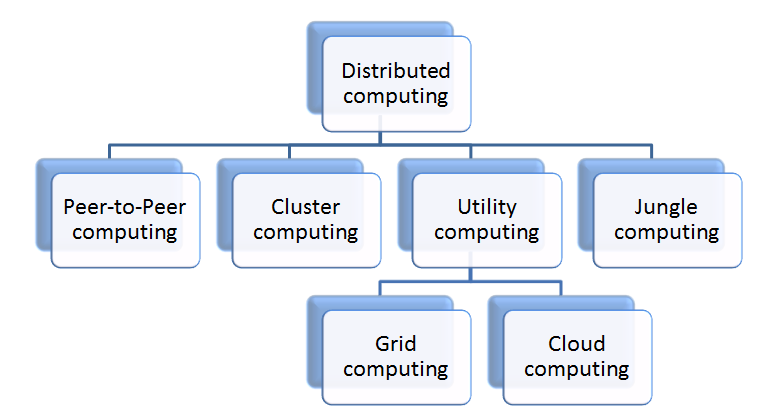
\includegraphics[scale=0.6]{DistributedComputingEnv.PNG}
\caption{Distributed Computing Environment}
\label{fig:DistributedComputingEnv}
\end{figure}

Each of the computing environment forming the part of the DCE is described briefly-
\begin{itemize}
\item \textbf{Peer-to-Peer computing}- Each node in the DCE acts as both client and server, providing as well as consuming part of the system resources. Peers are machines simply connected to the internet where in each peer can freely join and leave the DCE without affecting the whole system, implying no particular role(either master or slave) for a peer, making such a system self-organizing (figure \ref{fig:P2P}).

\begin{figure}[ht!]
\centering
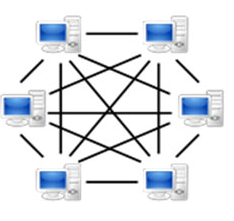
\includegraphics[scale=0.6]{P2P.PNG}
\caption{Peer-to-Peer system}
\label{fig:P2P}
\end{figure}

\item \textbf{Utility computing}- Utility computing is based on a model for service provisioning, which allows the users (consumers) to pay the providers for using the service only when they need to. It emphasizes on a business model, by which services provide make available the requested/paid resources to the costumers. All grid/cloud platforms are regarded as utility service providers. Grid computing is to enable coordinated resource sharing and problem solving in dynamic, multi-institutional virtual organizations where as cloud computing is a computing paradigm that involves outsourcing of computing resources with the capabilities of expendable resource scalability, on-demand provisioning with little or no up-front IT infrastructure investment costs. Cloud computing offers its benefits through
three types of service or delivery models namely infrastructure-as-a-service (IaaS), platform-as-a-service(PaaS) and software-as-a-Service (SaaS) 

\item \textbf{Cluster Computing}- A cluster comprises a set of independent or stand-alone computers and a network interconnecting them. It
works cooperatively together as a single integrated computing resource. A cluster is local in that all of its component subsystems are supervised within a single administrative domain, usually residing in a single room and managed as a single computer system. The components of a cluster are connected to each other through fast local area networks. 

\item \textbf{Jungle Computing}- It is the combination of one or more DCEs enlisted above resulting in a highly diverse, distributed and non-uniform high performance computing environments (figure \ref{fig:JungleComputing}).  

\begin{figure}[ht!]
\centering
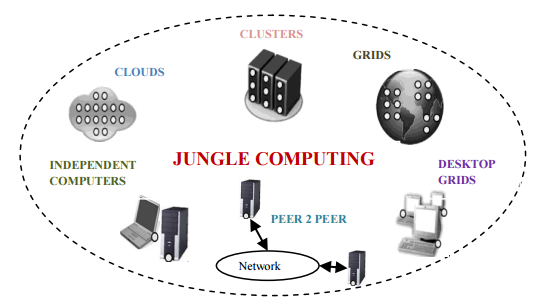
\includegraphics[scale=0.6]{JungleComputing.PNG}
\caption{Jungle Computing}
\label{fig:JungleComputing}
\end{figure}

\end{itemize}

